% vim: expandtab tabstop=2 softtabstop=2 shiftwidth=2
\documentclass[aspectratio=169]{beamer}
\usepackage[english,noconfigs]{babel}
\usepackage{ifluatex,ifxetex}
\ifnum 0\ifxetex 1\fi\ifluatex 1\fi=0 % if pdftex
  \usepackage[utf8]{inputenc}
  \usepackage[T1]{fontenc}
\fi

\usepackage{beamertpt}
\graphicspath{{graphics/}}

\usepackage{tikz}
\usetikzlibrary{trees}

\setbeamercovered{transparent=15}

\title[Pattern-based prediction algorithms, applications and variations]
      {Universal predictor}
\author{%
  Carolina de Senne Garcia\\%
  Clément Durand%
}

\renewcommand{\arraystretch}{1}
\setlength{\tabcolsep}{0.5ex}
\setlength{\fboxsep}{0.4ex}

\colorlet{fboxcolor}{white}
\newcommand\cfbox[1]{%
  \colorlet{currentcolor}{.}%
  {\color{fboxcolor}\fbox{\color{currentcolor}#1}}%
}

\begin{document}
\maketitle

\begin{frame}{Roadmap}\Large
  \begin{itemize}
    \item Algorithms
      \begin{itemize}
        \item Simplified predictor
        \item Universal predictor
        \item Variation proposal
      \end{itemize}
    \item Experimentation \& comparison
  \end{itemize}
\end{frame}

\tptsection{Simple predictor}

\begin{frame}{Algorithm and Implementation}
  \begin{itemize}
    \item \textbf{Basic idea}: find the longest suffix match in the given string (that is not a suffix itself)
  \end{itemize}

  \vspace{\fill}

  How we coded it:
  \begin{itemize}
    \item \textbf{Match pattern end indexes}: stored in a set
    \item \textbf{Scan set} to find longer matches until none is found
  \end{itemize}
  \vspace{\fill}

    Always better with an example...

\end{frame}

\begin{frame}{Example}\centering
  \input{code/simplified.tex}
\end{frame}

\tptsection{Universal predictor}

\begin{frame}{Algorithm and Implementation}
   \begin{itemize}
    \item \textbf{Basic idea}: use previous idea to calculate maximal length $L$ of mathing pattern suffix. Then take the set of matches of length $\alpha \cdot L$ and return the character following those sequences with higher frequency.
  \end{itemize}

  \vspace{\fill}

  How we coded it:
  \begin{itemize}
    \item \textbf{Match pattern end indexes}: stored in a list of sets. Each set corresponds to one length
    \item \textbf{Scan last set in the list} to find longer matches until none is found
    \item Use \textbf{set with matches of length $\alpha \cdot L$} to determine which following character is the most frequent
  \end{itemize}
  \vspace{\fill}

    Always better with an example...

\end{frame}

\begin{frame}{Example}\centering
  \input{code/complete.tex}
\end{frame}

\tptsection{Variation proposal}

\begin{frame}{Algorithm and Implementation}
   \begin{itemize}
    \item \textbf{Basic idea}: Precompute a substring tree. Then looking for suffix matches during the prediction is much faster.
  \end{itemize}

  \vspace{\fill}

  How we coded it:
  \begin{itemize}
    \item \textbf{Define a parameter p} for the maximum length of substrings (hence maximum height of the tree)
  \end{itemize}
  \vspace{\fill}

    Always better with an example...

\end{frame}

\begin{frame}{Reading substrings}\centering
  \input{code/learning.tex}
\end{frame}

\tptsection{Experimentation}

\begin{frame}{Parameters influence}
 \begin{table}
    \centering
    \begin{tabular}{c || c  c}
      $\alpha$ & Lorem Ipsum & Bible \\\hline\hline
      1.0 & 58.97\% & 65.67\% \\\hline
      0.9 & 59.19\% & 65.30\% \\\hline
      0.8 & 59.26\% & 65.52\% \\\hline
      0.7 & 59.26\% & 65.30\% \\\hline
      0.6 & 57.58\% & 61.13\% \\\hline
      0.5 & 56.55\% & 64.10\% \\\hline
      0.4 & 51.78\% & 61.61\% \\\hline
      0.3 & 43.21\% & 57.21\% \\\hline
      0.2 & 34.90\% & 53.12\% \\\hline
      0.1 & 27.18\% & 44.82\%
    \end{tabular}
    %\caption{\label{alpha} Precision performance for different $\alpha$ values applied to Lorem Ipsum and an extract from the Bible}
  \end{table}
\end{frame}

\begin{frame}{Distributed design}\centering
  \only<1>{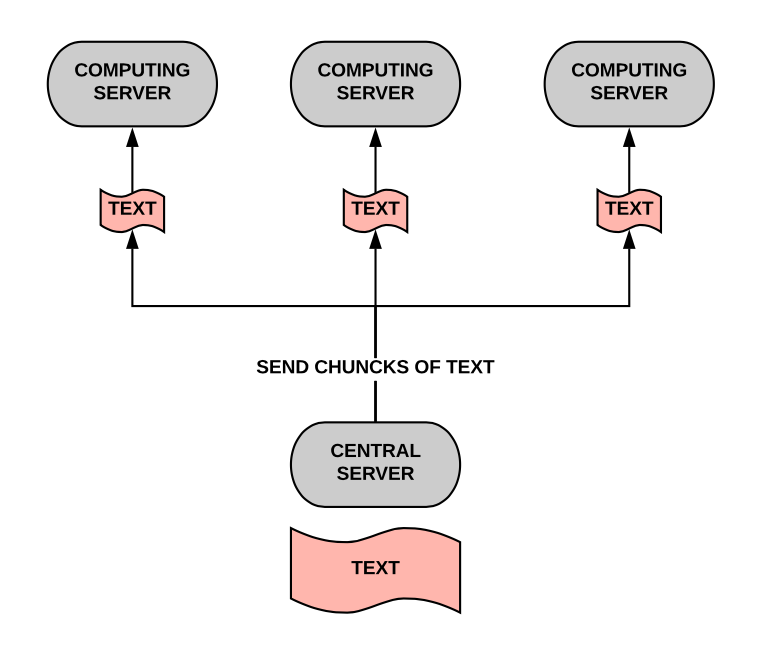
\includegraphics[height=.8\paperheight]{images/distributed1}}%
  \only<2>{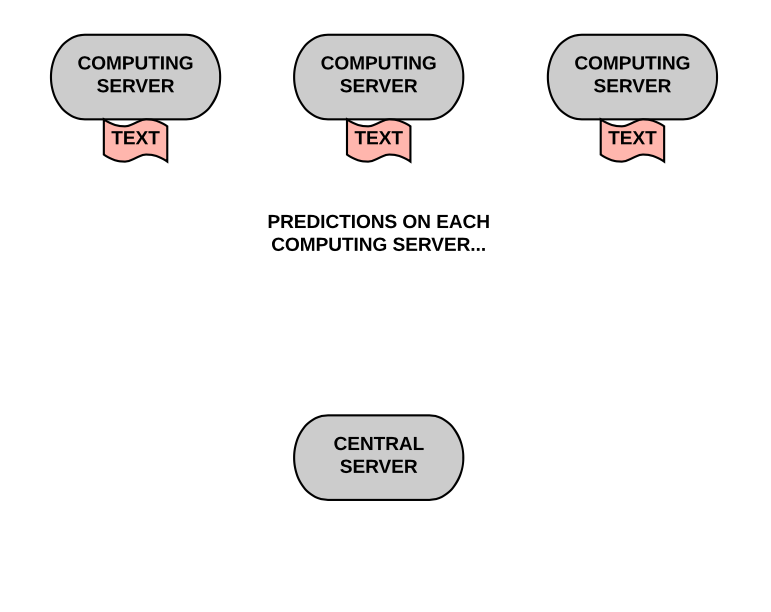
\includegraphics[height=.8\paperheight]{images/distributed2}}%
  \only<3>{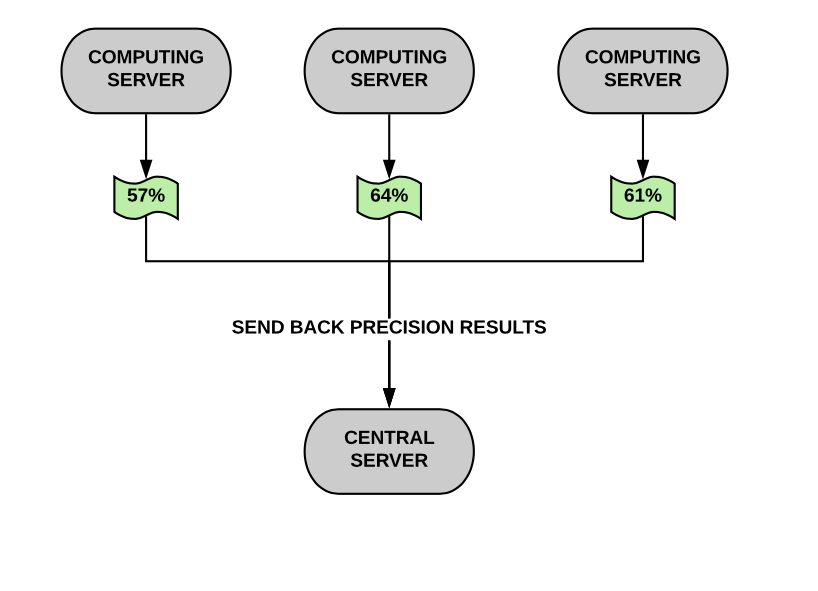
\includegraphics[height=.8\paperheight]{images/distributed3}}%
  \only<4>{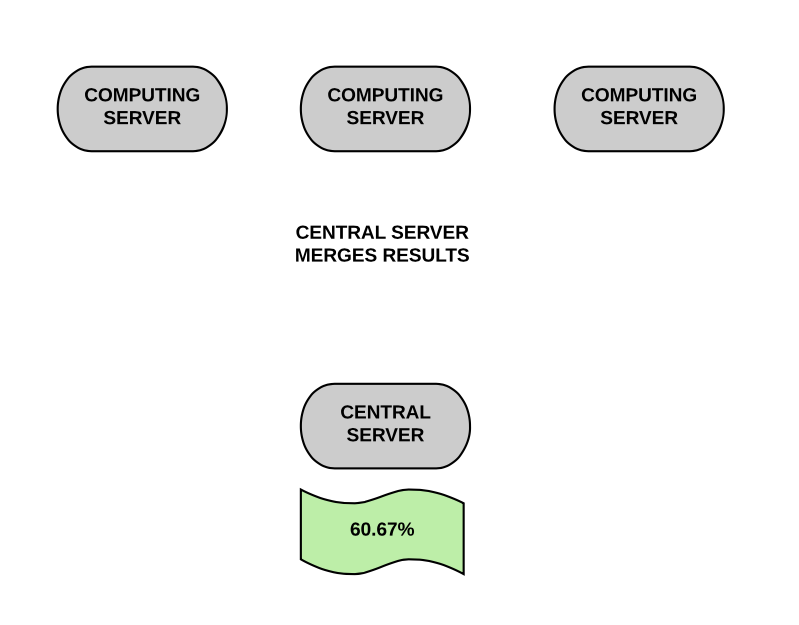
\includegraphics[height=.8\paperheight]{images/distributed4}}%
\end{frame}

\tptsection{Comparison}

\begin{frame}{Time and Memory Complexity}
  \begin{itemize}[<+->]
    \item \textbf{Learning algorithm} is faster to predict, but\ldots
    \item \textbf{Precomputation} required is long and used \textbf{memory space} is large!
  \end{itemize}
\end{frame}

\end{document}
